\chapter{Patterning in Synthetic Bacterial Colonies} \label{chapter3}
Using the insights obtained in the previous chapter, a wide range of microscopy experiments were carried out in optimal Turing conditions to obtain patterning in \textit{E.~coli} biofilms.
The aim is to observe fluorescent periodic patterns when these biofilms are observed under the microscope.
The model is key to elucidate which mechanisms are actually behind the patterns, and specifically to investigate if periodic patterns obtained are a result of Turing's mechanism.

In this section, experimental results produced in this thesis are shown.
Further microscopy results done by researchers at the Isalan Lab are also presented.
A framework to numerically solve reaction-diffusion systems in shaped and growing biofilms is developed to compare model outputs and experimental results.
Finally, perturbation experiments are carried out computationally, to predict experimental perturbations and elucidate the mechanisms of pattern formation.

\section{Experimental rings in small colonies with high aTc}\label{Rings in small colonies with high aTc}
In the previous chapter, certain conditions which could affect robustness for Turing pattern formation were found.
As already shown, the circuit components were matched by Dr.~Jure Tica and Tong Zhu (see Fig~\ref{fig:dose_response_experimental}) to improve robustness as seen in Fig.~\ref{fig:balancing_robustness}.
In this section, I investigate the circuit in a biofilm using confocal microscopy under the optimal Turing conditions obtained in Chapter~\ref{chapter2}.
More specifically, I look at how the biofilm fluorescent patterns change with different levels of aTc in small colonies

MK01 \textit{E.~coli} cells were transformed using electroporation (Section~\ref{electroporation}) with the full circuit.
This involved the introduction of 4 plasmids with the three nodes and the regulator cassette as seen in Fig.~\ref{fig:synthetic circuit_chapter2} and Table~\ref{tab:plasmid table} into our \textit{E.~coli} cells.
For this, the cells were then plated in 6 well MatTek plates and grew as individual colonies which are radially growing biofilms.
These growing colonies are then imaged using confocal microscopy.
Confocal microscopy is a type of fluorescence microscopy used to image thicker objects, where the beam of light focuses on one depth level, meaning you can get a single z-plane of fluorescence.
This way we can obtain a 2D fluorescence pattern steaming from a single focal plane of the colony ~\parencite{semwogerere2005confocal}.
 Detailed methods on colony plating and microscopy can be found in Section~\ref{microscopy}.
Red and green channels were imaged to detect mCherry and GFP as seen in Fig.~\ref{rgchannels}A,B.
These channels can then be superposed to get a GFP-mCherry combined reading (Fig.~\ref{rgchannels}C).
\begin{figure}[H]

    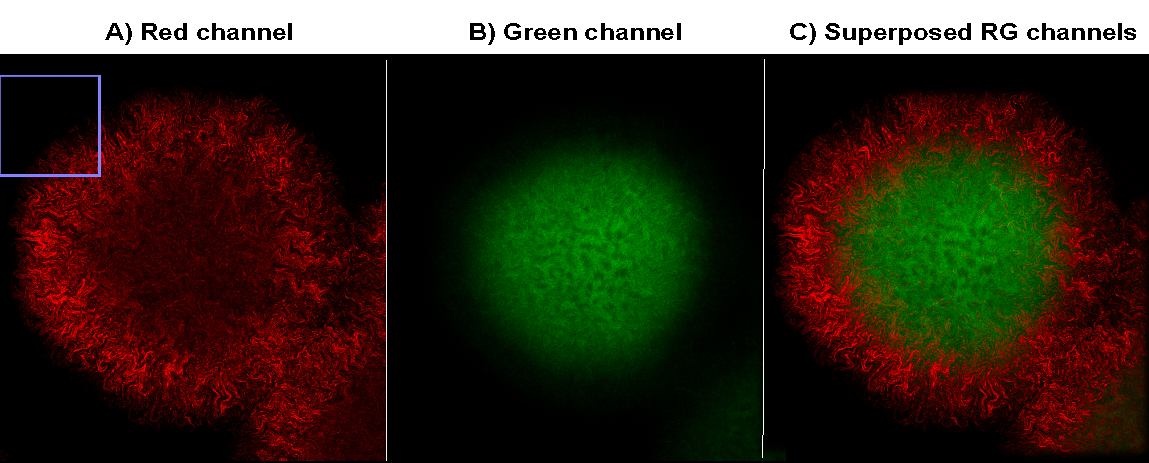
\includegraphics[width=1\textwidth]{chapters/Chapter 3/rgchannels}
    \caption{\textbf{2D plane of \textit{E.~coli} bacterial colony transformed with \#1754 synthetic circuit.} Image obtained with confocal microscopy. \textbf{(A),(B)} Red and green fluorescence channels with relative fluorescent units show the normalised concentrations of GFP and mCherry. \textbf{(C)} The superposed channel contains both red and green channels showing red at the edge and green at the centre.}
    \label{rgchannels}
\end{figure}

To test the impact of aTc on the patterning of the circuit, we prepared the agar on the MaTek plates with different levels of aTc, ranging from 0 to $10^1 \mu M$.
Different colony patterns arise from this aTc 'walk' as seen in Fig.~\ref{atcwalk_timeseries_confocal}A.
The colonies exhibiting more spatially heterogeneous behaviour are those with high aTc ($10^1 \mu M$).
This high aTc condition is further explored by imaging every day.
In Fig.~\ref{atcwalk_timeseries_confocal}B, we see how over time, the center of the colony oscillates from black to red to green.
As this happens, rings get added from the centre as in~\cite{Konow2019}'s interior ring growth mechanism.
The final snapshot (64h) shows green, red, green, red progression starting from the centre.
High DAPG conditions were also tested, as the model predicted this could also increase the likelihood of Turing patterns.
However, unlike with aTc, no patterns were observed with a high DAPG concentration.
\begin{figure}[H]

    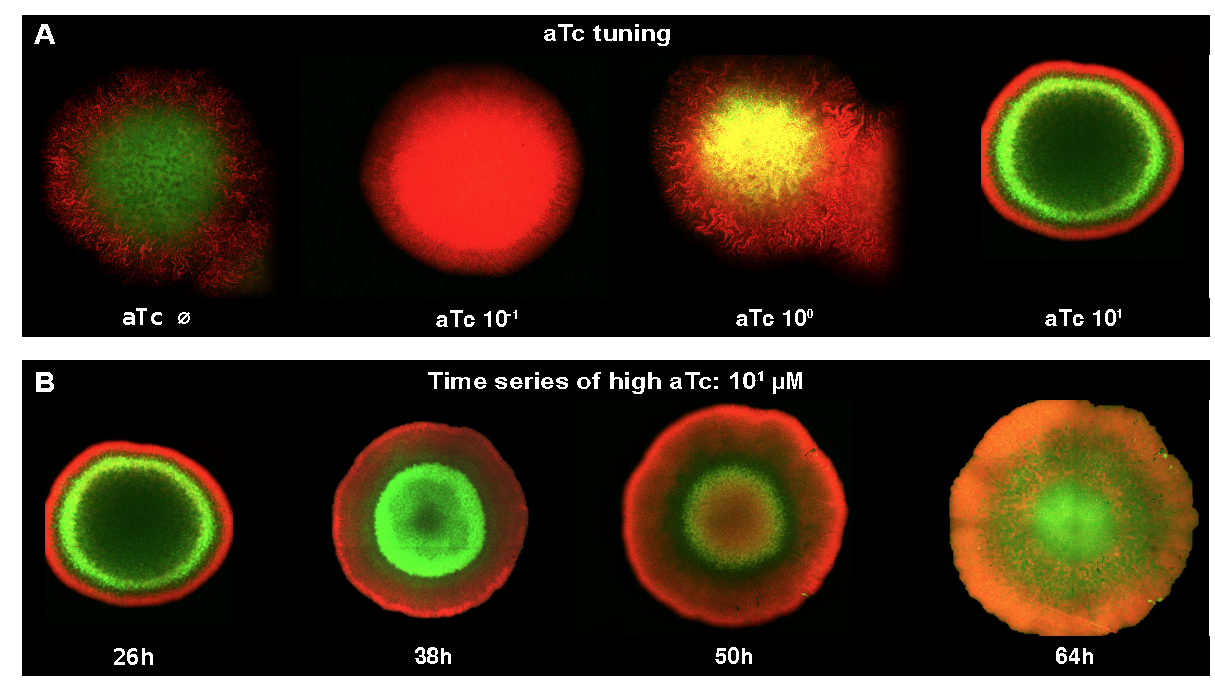
\includegraphics[width=1\textwidth]{chapters/Chapter 3/atcwalk_timeseries_confocal}
    \caption{\textbf{Confocal images of small colonies with gene circuit \#1754}. \textbf{(A)} Colonies with different aTc conditions at time 26h: no aTc $10^{-1} \mu M,10^{0} \mu M,10^{1} \mu  $. \textbf{(B)} Time series of single colony with high aTc condition ($10^1 \mu M$). Interior ring growth dynamics can be observed. The centre oscillates from black (26-38h) to red (50h) to green (64h). The black centre and the red centre become rings at the next time point. }
    \label{atcwalk_timeseries_confocal}
\end{figure}

Following this work, we continued studying this synthetic patterning system more in-depth.
Two routes were followed.
The first one involved specific shaped domains achieved by imprinting the agar with bacteria using shaped objects (Fig.~\ref{shmoo}).
The aim was to understand how the pattern adapts under different shaped domains.
The second route, and most explored, involved larger colonies to determine whether more repeats would form in a Turing-like behaviour.
This was achieved by carefully diluting the sample and plating a single colony without any neighbours.

\section{Modelling framework for synthetic circuit in bacterial tissues}
Most theoretical studies which involve Turing patterns, numerically simulate their system using square domains with no-flux or periodic boundary conditions.
However, these numerical domains are often not biologically realistic.
For example, the system we have developed experimentally involves more specific conditions including shaped domains, stochastic growth and absorbing boundary conditions.
To have a predictable model of our experimental system, the numerical solver had to be adapted to include such domain characteristics.

\subsection{Alternating Direction Implicit Method with defined domains}\label{Alternating Direction Implicit Method with defined domains}
All simulations in this chapter are performed in a \acrshort{2D} space to match the \acrshort{2D} focal plane captured by the confocal microscopy.
For this purpose, the numerical solver schema  \acrfull{ADI} is used.
This numerical solver produces a 2D space solution in time for the $n$ number of species of the model.
This method is chosen over \acrshort{CN} used in the previous chapter, as it is more efficient to solve 2D problems due to the matrix diagonalisation (see Section~\ref{numerical_methods}). More specific details of ADI can be found in Section~\ref{ADI}.



ADI is originally defined to solve square domains.
To integrate our specific domains with the solver, a masking method is used where a "shape matrix" is passed containing the shape of the domain.
The "shape matrix" is a Boolean matrix of $IxJ$ size which contains information on the location of the cells.
1's determine cells, while 0's determine agar.
When passing this matrix to the solver, the algorithm computes reaction and diffusion terms in 1 positions while it only computes diffusion in 0's.
Fig.~\ref{mask}~right shows the "shape matrix" where 1's are black and 0's are white.
Additionally, this figure shows what functions are computed in which regions.
How the "shape matrix" is defined depends on the experimental setup.
Using this masking method, we will obtain a solution for the $n$ number of species of our model, in time and space, within the biofilm.

\begin{figure}[H]
    \centering

    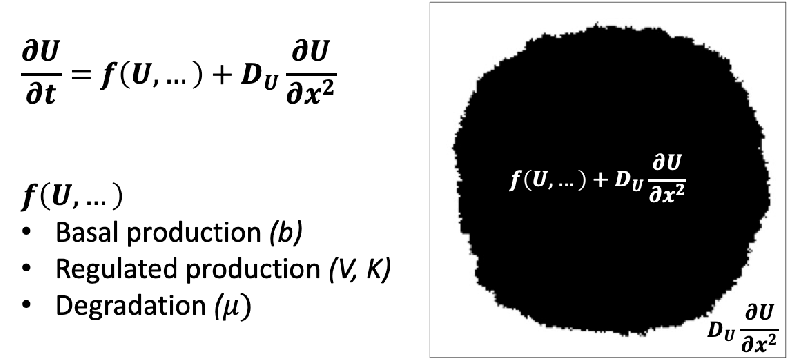
\includegraphics[width=0.9\textwidth]{chapters/Chapter 3/mask}
    \caption{\textbf{Masking of PDEs with tissue shape.} Our PDEs are composed of reaction and diffusion terms (left). The masking method (right) consists of computing the different terms of the PDE in different regions of the system. A shape matrix (square with a black circle) determines where the reaction and diffusion terms are computed (black) and where only the diffusion term is computed (white).}
    \label{mask}
\end{figure}

\subsection{Static Shaped domains}
Following the small rings produced in this thesis, Tong Zhu from the Isalan Lab started experimenting with non-circular domains.
Specific shapes were obtained by imprinting the agar with bacteria using shaped objects.
Fig.~\ref{shmoo}A shows the resulting biofilm after impregnating the agar with bacteria using the edge of a glass coverslip.
In this thesis, the biofilm shape is replicated by using a "shape matrix" derived from the microscopy image Fig.~\ref{shmoo}B.
This is done through image recognition on the microscopy snapshots to detect areas with cells (see Section~\ref{Tissue area recognition}).


\begin{figure}[H]
    \centering

    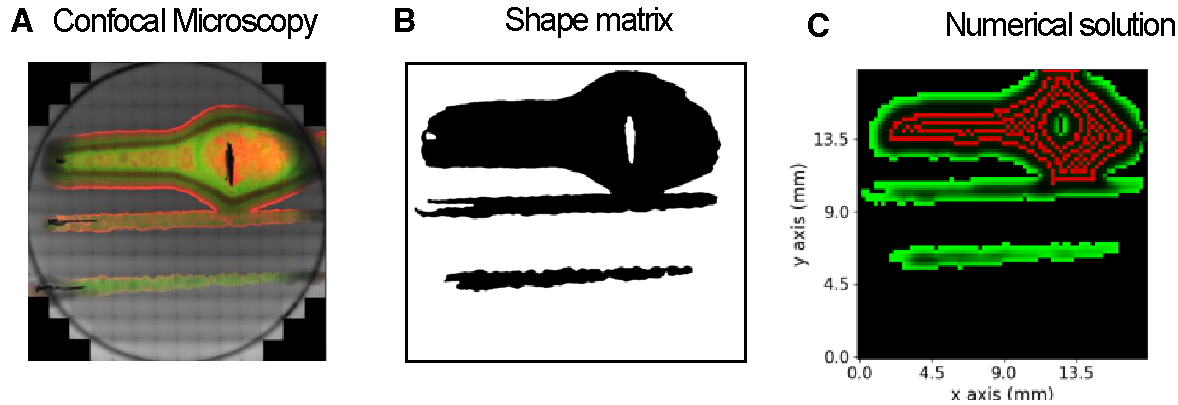
\includegraphics[width=1\textwidth]{chapters/Chapter 3/shmoo}
    \caption{\textbf{Image recognition of confocal microscopy image for PDE masking.} \textbf{(A)} Confocal microscopy of three \textit{E.~coli} biofilms grown by seeding with the edge of a glass coverslip. This experiment was done by Tong Zhu. \textbf{(B)} Shape matrix obtained using image recognition on biofilm in (A) to detect cells. Black shows cells while white shows agar. \textbf{(C)} Numerical solution of six-equation model with a Turing parameter set, using the masking method with the shape matrix in (B).}
    \label{shmoo}
\end{figure}
Using the masking method with ADI explained in ~\ref{Alternating Direction Implicit Method with defined domains}, a numerical solution was computed within the defined biofilm.
The PDE system used is the six-equation model (Eq.~\ref{[6 equation proteins]}), which describes synthetic circuit \#1754, using a Turing parameter set found through linear stability analysis.
The numerical solution is shown in Fig.~\ref{shmoo}C as a superposition of the red and green channels.
Details on how to plot the numerical solution of the six-equation as a red-green image like confocal microscopy can be found in Section~\ref{Plotting superposed numerical solution as confocal microscopy results}.
The stripes obtained with the Turing model adapt to the shape of the tissue.
Some stripes with the same adaptation to the tissue shape can be observed in the confocal microscopy experiment (Fig.~\ref{shmoo}A).
This shows the importance of modelling tissue shape in Turing patterns.

\subsection{Growing colony with cellular automaton}
Most of the work we carried out experimentally to explore the system was done in bacterial colonies.
These colonies are radially growing biofilms with stochastic cell division.
Therefore, the static image recognition method used above is not suitable as we do not have time-series confocal data for most samples to create a dynamic "shape matrix".
To recreate the dynamic behaviour of the colony growing, a stochastic growth model was developed using a cellular automaton.

A cellular automaton is a discrete model of computation constructed with a few basic rules ~\parencite{gardner1970mathematical}, which can accurately describe how the shape of the bacterial colony evolves over time.
As the "shape matrix", the cellular automaton consists of a Boolean 2-dimensional matrix, where grid points can be in a cell (1) or agar (0) state.
This Boolean matrix evolves over time when the following three rules are applied: If a cell (1) grid-point has any agar (0) neighbours, it will divide into the neighbouring agar (0) gridpoint with a probability $p_{d}$.
No cell death (1 to 0 transition) is permitted.
Newborn cells inherit the full concentration of their mother cells.
This last assumption is taken as mRNA transcript homeostasis ensures the concentration of mRNAs is maintained at cell division and as cell size increases by scaling between transcription rates and cell size ~\parencite{berry2022mechanisms,volteras2023global}.
Because we are modelling protein concentration, we can then assume that mRNA concentration is linearly correlated with protein concentration for synthetic genes like ours.
If some dilution occurs, this can be accounted for in the degradation terms of the PDE model.

To model a single colony, a 0's matrix is initialised with a 1 in the middle, describing the first cell as it occurs in single-cell colonies.
When the cellular automaton rules are applied to this initial matrix, a circular cell domain starts growing stochastically, resembling a bacterial colony (see Fig.\ref{cas}A-B).
The division process consists of a probabilistic process where division occurs or not based on a probability of division ($p_{d}$).
The division process is iteratively applied to the matrix until the final time (T) is reached.
The computation is applied every ‘m’ hours, so
\begin{equation}
        T = \sum_{n=1}^{T/m} m\cdot n
\end{equation}

e.g. if $m=0.2$ at $T=0.2, 0.4, 0.6 \ldots etc$ .
The growth rate can be tuned by increasing the probability of division ($p_d$) or decreasing $m$, so it matches the experimental growth rates.
Linear growth curves are obtained for the simulations with the cellular automata, similar to the experimental ones (see Appendix~\ref{appendix_growth_rates}).
Furthermore, different $p_d$’s can be applied to different regions of the matrix to achieve faster-growing subregions within the colony (see Fig.~\ref{cas}C).
Finally, to simulate two colonies, two 1’s are placed at a distance (see Fig.~\ref{cas}D).

\begin{figure}[H]
    \centering

    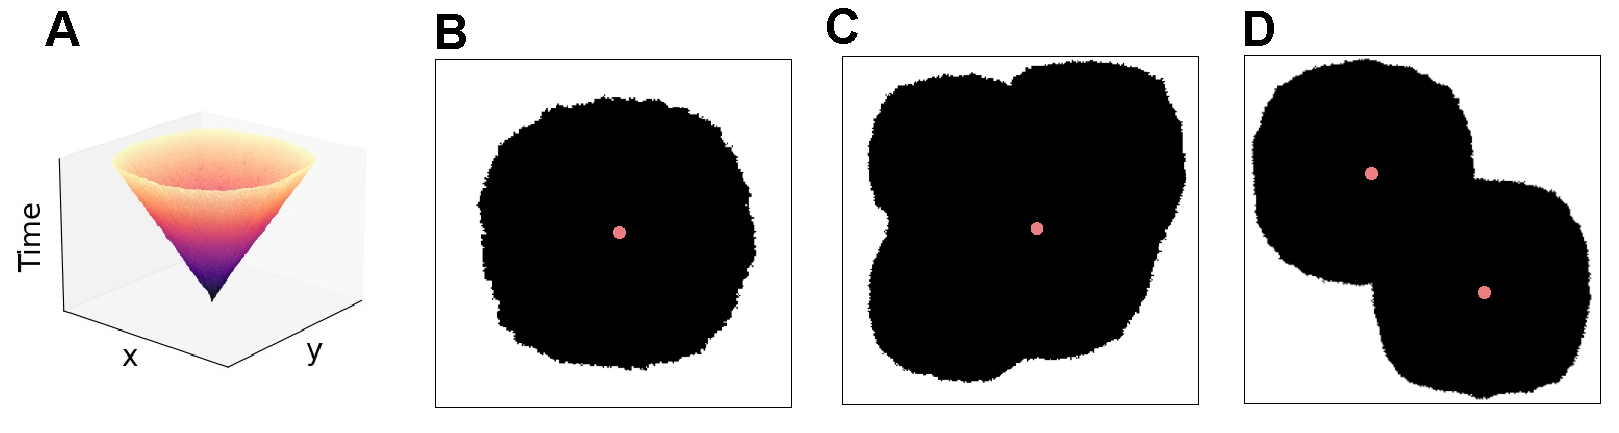
\includegraphics[width=1\textwidth]{chapters/Chapter 3/cas}
    \caption{\textbf{Stochastic model of colony growth with cellular automaton.} \textbf{(A)} Time series of colony growth in 2D. Purple depicts older cells, while yellow shows newer ones. \textbf{(B)} Final snapshot of a colony growing with growth rates homogeneous throughout the colony. \textbf{(C)} Final snapshot of a colony growing with different rates throughout the colony. \textbf{(D)} Two colonies growing and merging with homogeneous growth rates. Black shows cells, white shows agar and the pink dot shows the initial cell from which the colony grows.   }
    \label{cas}
\end{figure}
The masks obtained can be used to compute the solution of the PDE in the biofilm.
Unless otherwise stated, a reflective boundary condition (Neumann) is used at the edge of the square where the agar finishes.
Taking an arbitrary parameter set, this method produces a numerical result similar to that of the colonies obtained in Section~\ref{Rings in small colonies with high aTc}.
The comparison can be seen in Fig.~\ref{small colony experiment vs model} where the red edge with green centre is reproduced.
This pattern, which is commonly seen throughout, most likely stems from the boundary effects at the edge of the colony which is captured by the masking method.

\begin{figure}[H]
    \centering

    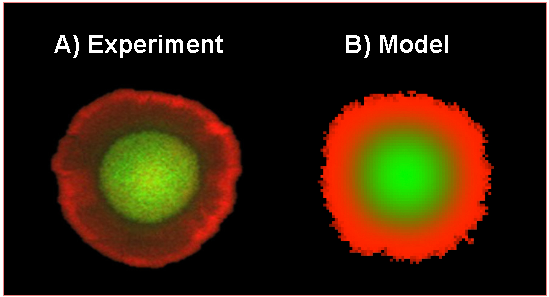
\includegraphics[width=0.6\textwidth]{chapters/Chapter 3/small colony experiment vs model}
    \caption{ \textbf{PDE model with colony growth replicates experimental colonies} \textbf{(A)}~Red-green superposition image of small E.coli colony with circuit \#1754.  \textbf{(B)} Numerical solution of masked PDE using a cellular automaton colony growth model. Both images show a colony with a red edge and a green center.}
    \label{small colony experiment vs model}
\end{figure}

\subsection{Adapting time and space in the dimensionless model}
When solving our system numerically, time and space are key parameters that define the bounds of our simulation.
As seen in the previous chapter, time and space are dimensionless and dependent on the model’s parameters
\begin{equation}\label{time_space_transform}
    t = \frac{t*}{\mu _a}, \quad x = \sqrt{\frac{k_{1}D_{u}}{\mu_{a}\mu_{u}}}x^*
\end{equation}

When sampling the parameter space, the parameters related to time and space transformations are fixed, so $\mu_a = 0.3 \,h^{-1}, \,k_1 = 0.0183 \,h^{-1},\, \mu_u = 0.0225\, h^{-1}$.
The diffusion rate $D_U$ is the only one not fixed and it ranges from $0.1-10 \,mm^2h^{-1}$.
Using Eq.~\ref{time_space_transform}, time is transformed so that $t^*=3.3\cdot t$.
Space is also transformed but is dependent on $D_U$, which is sampled from a range.
Therefore, for $D_U = [0.1, 10] \,mm^2 h^{-1}$, $x^* =[1.92 - 0.192] \cdot x$.
Using realistic experiment time and space, the following dimensionless values are obtained:
For time $t=166\,h$, dimensionless time $t^*=50$.
Dimensionless space  $x^*=16$ is taken so  $x = [8.32, 83.2] \,mm$, with $D_U = [0.1, 10]\, mm^2 h^{-1}$ respectively.
These values of t and x lie within realistic physical parameters for our system.
These transformations are dependent on parameters that may vary experimentally, and therefore some uncertainty must be allowed.
The experimental values used here are an example of how to carry out the transformations, however all simulation parameters for space and time can be found on Tables~\ref{tab:model_param1},~\ref{tab:model_param2},~\ref{tab:numerical_param_table}.

The space resolution taken is $dx^*=0.1$.
If transformed to non-dimensional units, this would be $dx =[0.052-0.520] mm = [52-520] \mu m$.
This means that the biological size of every pixel of the simulation varies from $52\mu m$ to $5200\mu m$ depending on the $D_{U}$ chosen.
Because the model is dimensionless, the spatial resolution is lower if a higher diffusion constant for U is used.
If we assume an \textit{E.~coli} cell has a size of around $~1\mu m$~\parencite{shiomi2009genetic}, in every pixel there are around 52 to 5200 \textit{E.~coli} cells.
\section{Colony pattern dynamics in parameter space searches}

The experimental work in this thesis produced the first rings observed in the system, where small colonies were used (Section~\ref{Rings in small colonies with high aTc}).
Following this, experiments were carried out in larger colonies by Dr.~Jure Tica, Tong Zhu, Dr.~Georg Wachter and Dr.~Dario Bazzoli from the Isalan Lab.
From here onwards, all experimental results were produced by them unless otherwise stated.
A wide variety of patterns were produced by growing larger colonies.


\subsection{Circuit exploration in literature-based distribution}
In parallel to microscopy work, the model predicted a wide variety of patterns could be produced in different dynamical regimes, which matched the experimental variability.
This was shown by exploring the parameter space of our circuit within literature-based ranges.
The distribution used is described in Section~\ref{Definition of parameter space based on literature parametrisation} and more specifically Table~\ref{tab:literature param distributions}.
In this exploration, linear stability analysis was carried out and outputs were classified following linear stability classification in Fig.~\ref{fig:dispersions}.
The frequencies in parameter space of the linear stability solutions are shown in Fig.~\ref{system_class_frequencies}.
\begin{figure}[H]
    \centering

    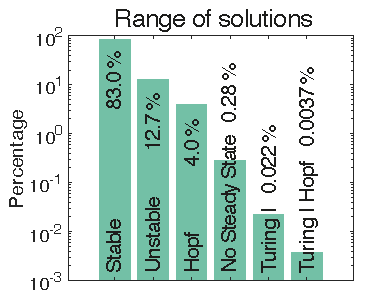
\includegraphics[width=0.6\textwidth]{chapters/Chapter 3/system_class_frequencies}
    \caption{\textbf{Types of dispersion relation solutions in literature-based distribution.} The frequency in parameter space for every type of dispersion is shown in terms of the percentage of sampled parameter sets.}
    \label{system_class_frequencies}
\end{figure}

Examples of different linear stability analysis outputs were then solved numerically, masked by a growing colony obtained with the cellular automata algorithm.
The different final pattern snapshots and time series can be seen in Fig~\ref{system_class_simulations}.
A wide variety of patterns and dynamics is observed including stationary rings, travelling waves, stationary and non-stationary spots, labyrinths and bistability wedges.
This global model analysis, with biologically relevant parameters, showed that our circuit can produce a broad range of spatial patterns, together with spatially homogenous solutions.
Overall, Turing I hopf and Turing I patterns are the most interesting heterogeneities due to their periodicity and stationarity.
However, they are not very robust ($0.022\%$ and $0.0037\%$ respectively).
On the other hand, Hopf solutions also produce interesting heterogeneities which are sometimes periodic and seem to occur more robustly ($4\%$).
It is important to add that Turing I Hopf solutions seem to produce patterns more robustly in this chapter than in Chapter~\ref{Chapter 1}.
All of the patterns shown are single steady state systems so we can understand the individual and isolated behaviour of that dynamical system.
However, some interesting multistable systems are present such as the Turing-Hopf-Unstable system shown in Fig.~\ref{comparison_colonies_model_vs_experiment} Rings \#1.
\begin{figure}[H]
    \centering

    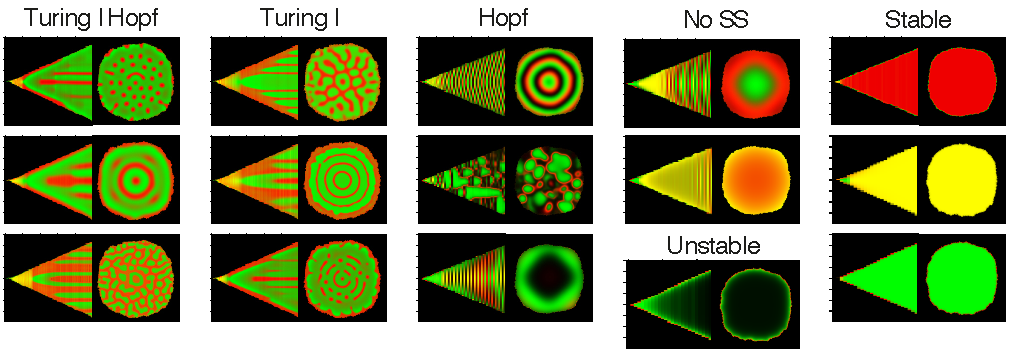
\includegraphics[width=1\textwidth]{chapters/Chapter 3/system_class_simulations}
    \caption{\textbf{Simulations of the hybrid PDE-bacterial colony solver for different types of dispersion relations}. The kymographs on the left show the time series of the colony cross-section. The plot on the right shows the final snapshot of the simulation. In both, the green and red channels are superposed. Turing I Hopf and Turing I solutions show stationary periodic patterns including outer ring addition. Hopf solutions show oscillatory solutions including interior ring growth.}
    \label{system_class_simulations}
\end{figure}


This wide variety of patterns was explored, and corresponding experimental solutions were found (see Fig.~\ref{comparison_colonies_model_vs_experiment}).
As the model predicted, the system can experimentally produce rings, spots, and wedges.
However, although labyrinths commonly appear in the model, they have not been found \textit{in-vitro}.


\begin{figure}[H]
    \centering

    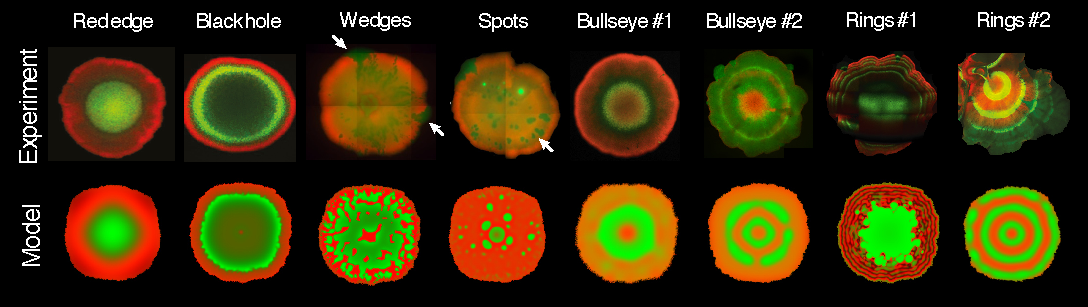
\includegraphics[width=1\textwidth]{chapters/Chapter 3/comparison_colonies_model_vs_experiment}
    \caption{\textbf{Variety of spatial patterns observed experimentally as well as in the model.} Various spatial patterns are observed when the full circuit is tested in growing colonies in different experimental conditions (upper row). The white arrows show two wedges and a region of spot formation. Colony size and tuning conditions are listed in Table S1. Patterns are reproduced with the circuit model (bottom row); for parameters see Suppl. Info. 4. All images except Red edge, Black hole and Bullseye \#1 can be attributed to Dr.~Jure Tica, Tong Zhu and Dr.~Georg Wachter. All parameters for these simulations can be found on Tables~\ref{tab:model_param1},~\ref{tab:model_param2},~\ref{tab:numerical_param_table}. The experimental conditions and colony sizes are shown in Table~\ref{tab:experiment_conditions}.}
    \label{comparison_colonies_model_vs_experiment}
\end{figure}


\subsection{Circuit exploration in liquid-culture fits distribution}
In the previous section, the model was explored using large literature-based distributions and was compared to experiments in a different range of tuning conditions.
In this section, we focus on a more constrained region of the parameter space obtained by fitting the model to liquid culture data (Section~\ref{Constrained parametrised distributions: fitting to liquid culture data of gene subcircuits}).
This parametrisation aims to explore a model which is better linked to the experimental system in terms of parameters and behaviour.
More specifically, this constraining is carried out to prove that the obtained experimental patterns exist in this fitted parameter space, in particular the more Turing-like concentric rings (Fig.\ref{comparison_colonies_model_vs_experiment} Rings \#2).


In Section~\ref{Fitting process and the resulting best fit distributions.}, the model was fitted to dose-response curves of subcircuits under high aTc and matched transfer functions conditions.
These are the same conditions where the Fig.\ref{comparison_colonies_model_vs_experiment} Rings \#2 appear.
As previously explained and shown in Fig.~\ref{fig:1d_distributions}, linear stability analysis was carried out on the fitted multivariate Gaussian distribution with $q=10$, and three Turing parameter sets were found.
These are the closest three Turing parameter sets to the best-fit solution.
Those three parameter sets were simulated using a colony growth mask (see Fig.~\ref{best_fit_colony_turing}).
Their dominant features include a central circular green (Case \#1) or red (Case \#2) spot, surrounded by a ring of green fluorescence, and a wedge or labyrinthian-like pattern.
These are all observed within the experimental data (see Fig~\ref{comparison_colonies_model_vs_experiment}).

\begin{figure}[H]
    \centering
    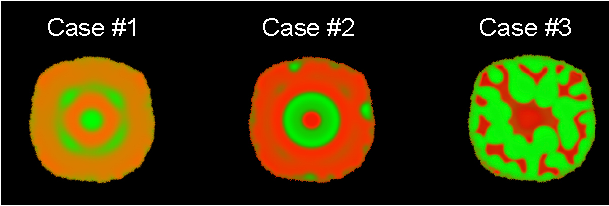
\includegraphics[width=1\textwidth]{chapters/Chapter 3/best_fit_colony_turing}
    \caption{Growing colony simulations of Turing solutions with fitted parameters. Parameters for these simulations can be found in Tables~\ref{tab:model_param1},~\ref{tab:model_param2},~\ref{tab:numerical_param_table}.}
    \label{best_fit_colony_turing}
\end{figure} %

Although Case \#1 seems to have similar rings to the ones we are looking to replicate (seen in Fig.\ref{comparison_colonies_model_vs_experiment} Rings \#2), more rings would be needed to prove that the periodic ring-like behaviour exists in the fit distribution.
Three routes can be taken to further explore the patterns present in the fit distribution.
The first one would be to explore different numerical parameters (e.g. space, time and growth rate) to obtain a different pattern.
However, numerical parameters are harder to explore from a computational parallelisation point of view.
The second one would be to sample more from the fit distribution to find more Turing parameters and simulate those.
However, Turing parameters are not commonly found and therefore it is also a computationally expensive task to obtain few results.
Finally, a third route exists which involves searching very closely around the vicinity of the already obtained parameter sets.
This route is chosen as it is the most efficient way of obtaining many Turing parameter sets that still belong to the fit distribution.

\subsection{Pattern exploration around the vicinity of Turing fit solutions}
The parameter space found around the fitted Turing parameter sets is explored. To do this, a small noise deviation is applied to the parameters with different levels of relative uncertainty.
For each parameter $p$, a normal distribution is generated with mean $\mu=p$ and standard deviation $\sigma=p\cdot u$. $u$ is the level of uncertainty which ranges from 0.01 to 0.2 (or 1\% to 20\% relative uncertainty).
This small noise perturbation to all parameters, which generates similar steady-state dose-response behaviour, allows us to further explore the Turing parameter space near the best fit to the liquid culture.

For each value of uncertainty, $2\cdot10^3$ parameter combinations were analysed.
The Turing patterning robustness with different amounts of noise is shown in Fig.~\ref{fig:turing_fit_noise_robustness}A, showing how robustness decreases as more noise in the parameters is added.
This figure shows how the local parameter space around Turing conditions is highly enriched with patterns (e.g adding a relative uncertainty of 1\% around a Turing I solution produces 33\% Turing I solutions, whereas an uncertainty of 5\% produces 5\% Turing I solutions).
The average relative uncertainty in the Vm and Km parameters between biological repeats in liquid culture data of Fig. 1b was 4.8\%.
This indicates that if a patterning region was found, Turing patterns could be sufficiently common to be reproduced.
The different analytical solutions for a relative uncertainty of 1\% are shown in Fig.~\ref{fig:turing_fit_noise_robustness}B, where we observe not only Turing I solutions, but also Turing I Hopf and Hopf solutions.
For this relative uncertainty (1\%), numerical solutions are computed and shown in Fig.~\ref{fig:turing_fit_noise_robustness}C.
Within the small vicinity of a ring-like Turing parameter set, we can find mainly rings and spots.
In particular, we can find solutions with multiple concentric rings such as the one marked with an arrow in Fig.~\ref{fig:turing_fit_noise_robustness}C Case\#4.

\begin{figure}[H] % h! is a placement specifier; it tries to place the image here.
    \centering
    \begin{adjustbox}{center}
        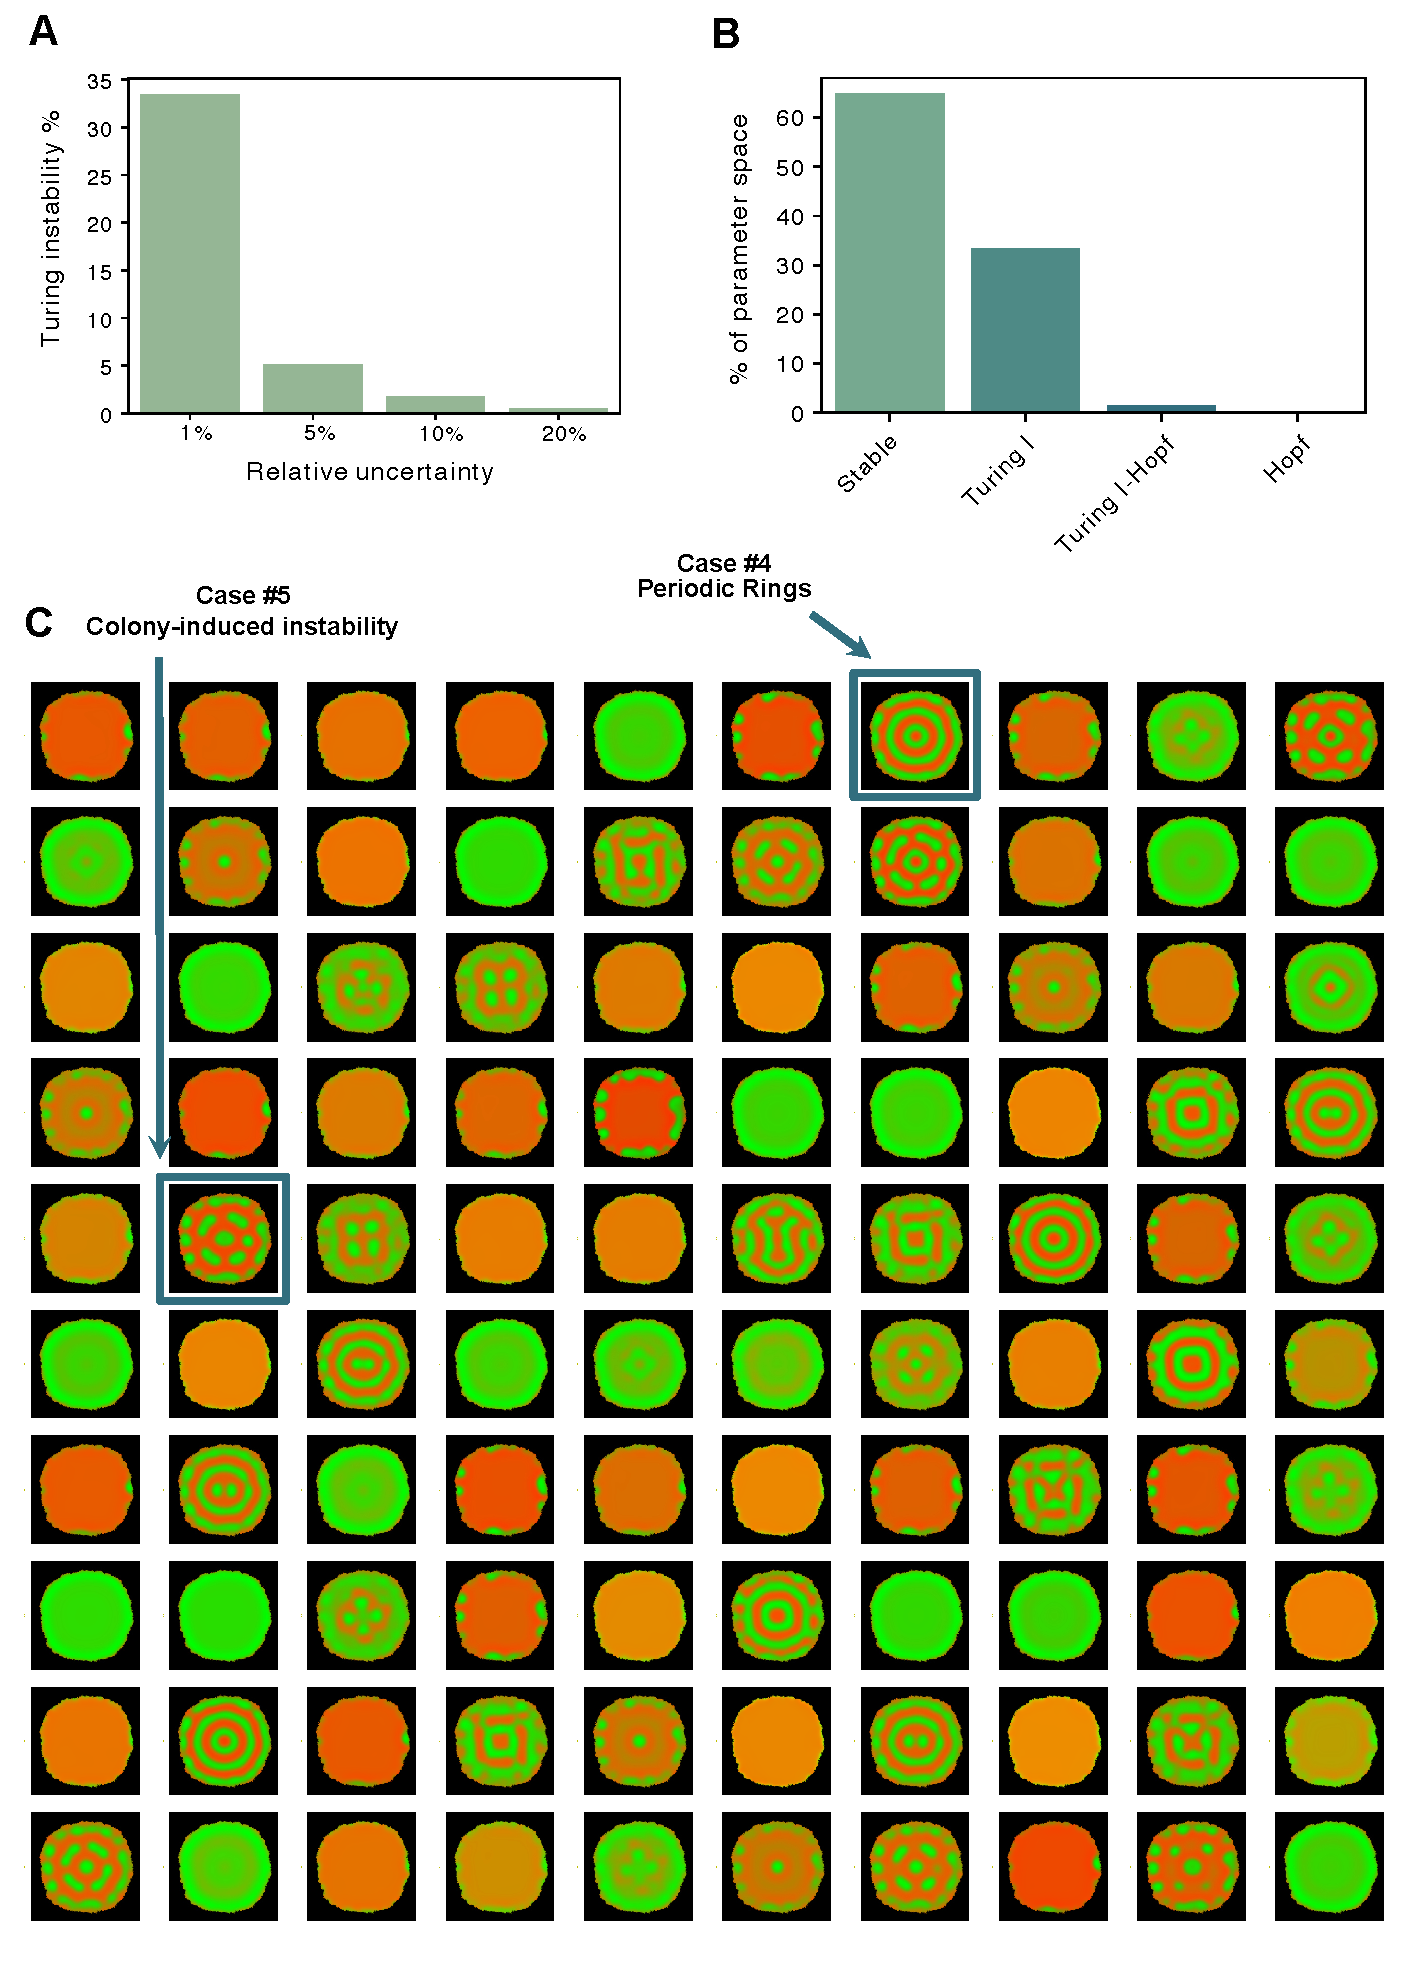
\includegraphics[width=1\textwidth]{chapters/Chapter 3/turing_fit_noise_robustness} % The name of your image file; assumes it is in the same directory as your .tex file
    \end{adjustbox}
    \caption{\textbf{Search around fitted Turing parameter set.} \textbf{(A)} Turing robustness with different levels of relative uncertainty. \textbf{(B)} Using 1\% relative uncertainty (mean $\mu=p$ and standard deviation $\sigma=p\cdot 0.01$), frequency of different analytical solutions: Simple stable 64.8\%, Turing I 33.5\%, Turing I-Hopf 1.5\%, Hopf 0.25\%. \textbf{(C)} Numerical simulations in growing colonies of 1\% noise distribution. Arrow points to Case \#4 which is a solution with multiple periodic rings and Case \#5 where a colony-induced instability is present.}
    \label{fig:turing_fit_noise_robustness}
\end{figure}

The time series of this particular Case \#4 Turing solution is explored and compared to different snapshots of the bacterial colony patterns.
Outer ring addition dynamics of both the model colony and the experimental colony are shown in Fig.~\ref{fig:outer_ring_addition_modelvsexperiment}, where rings get added to the edge of the colony.
One aspect to highlight is the diffusion ratio $Dr$ of this solution.
Assuming that the enzymatic production and degradation rates of the two diffusers pC and OHC14 are equal (k1 = k2, µU = µV), a Dr of 0.15 is very close to an experimentally measured Dr of 0.25~\cite{tica_diffusers}.

\begin{figure}[H] % h! is a placement specifier; it tries to place the image here.
    \centering
    \begin{adjustbox}{center}
        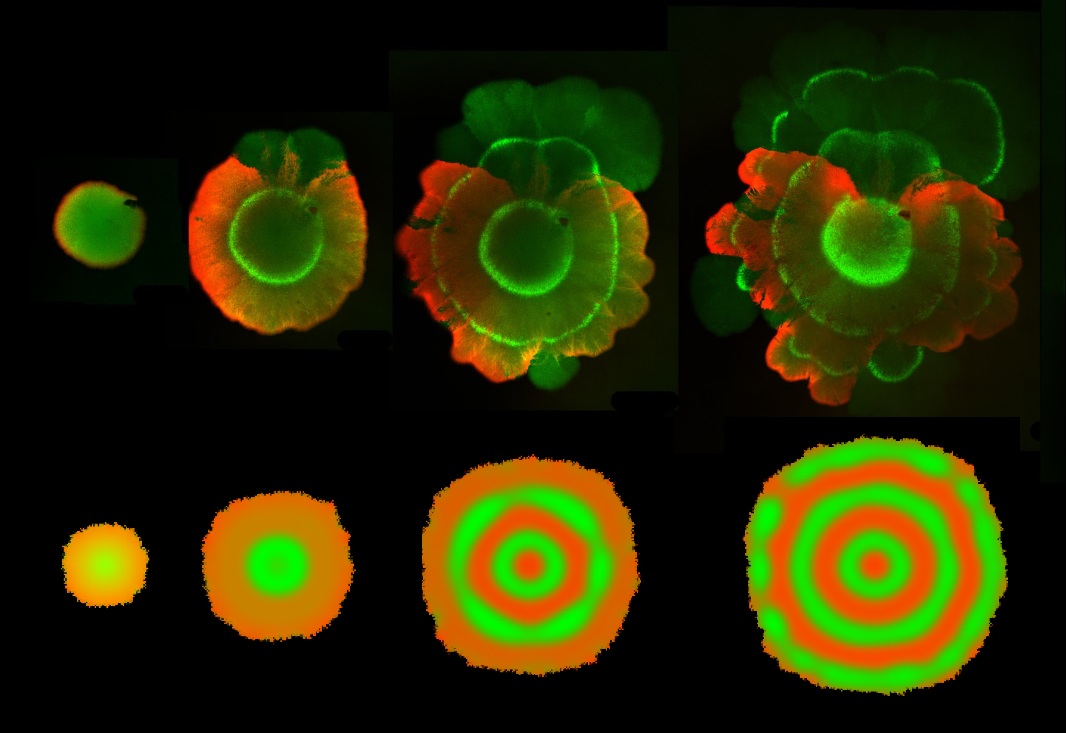
\includegraphics[width=1\textwidth]{chapters/Chapter 3/outer_ring_addition_modelvsexperiment} % The name of your image file; assumes it is in the same directory as your .tex file
    \end{adjustbox}
    \caption{\textbf{Time series of growing colony in experiment and model.} The top row shows confocal microscopy snapshots of the experiment at different time points. Image taken by Dr. Jure Tica. The bottom row shows the time series of the growing colony model. The model parameters used correspond to a Turing parameter combination found in the vicinity of the fitted distribution as seen in Fig.~\ref{fig:turing_fit_noise_robustness} Case \#4. In both experiment and model, a similar dynamic behaviour occurs where rings get added to the outside of the colony.}
    \label{fig:outer_ring_addition_modelvsexperiment}
\end{figure}

Other interesting solutions are found such as the colony-induced Turing pattern (Fig~\ref{fig:turing_fit_noise_robustness}C Case \#5).
In Fig.~\ref{fig:colony_induced_turing} we see an example of an instability induced by stochasticity in cell division or growth: the dispersion relation doesn’t show any unstable modes; however, the simulation shows a clear periodic heterogeneity.
The dominant mode of this dispersion relation (Fig.~\ref{fig:colony_induced_turing}A) has a wavenumber of 1.8, which corresponds to a wavelength of $2\pi/1.8=3.49$.
This approximately corresponds to the wavelength of the produced pattern (Fig.~\ref{fig:colony_induced_turing}B), meaning this stable mode has been excited to unstable and resulted in a Turing pattern.


\begin{figure}[H] % h! is a placement specifier; it tries to place the image here.
    \centering
    \begin{adjustbox}{center}
        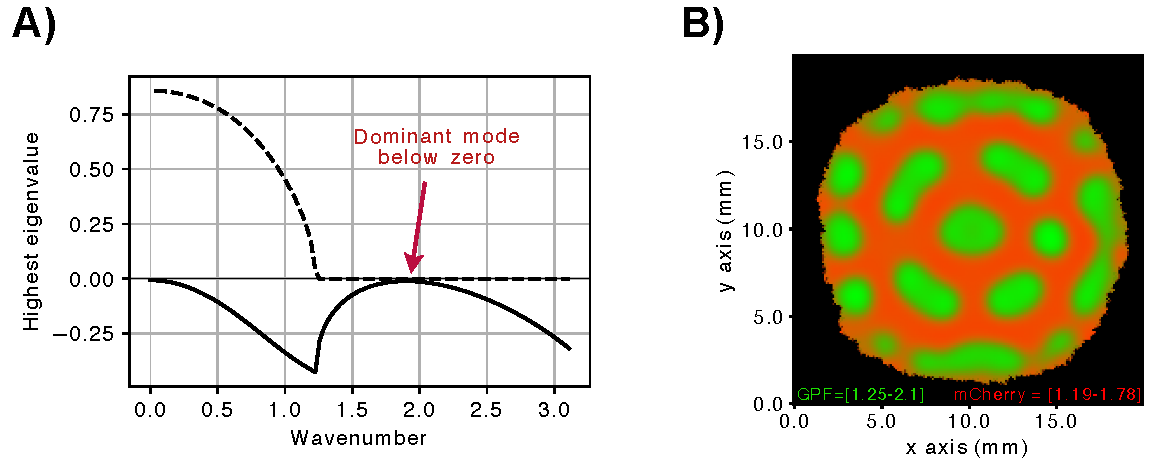
\includegraphics[width=1\textwidth]{chapters/Chapter 3/colony_induced_turing} % The name of your image file; assumes it is in the same directory as your .tex file
    \end{adjustbox}
    \caption{\textbf{Colony-induced instability.}  \textbf{(A)} Dispersion relation showing a stable system. The most dominant mode (wavenumber=1.8, wavelength=3.49). \textbf{(B)} Regular pattern is observed in the numerical solution of a stable system with dominant mode just below zero. The model parameters used correspond to a Turing parameter combination found in the vicinity of the fitted distribution as seen in Fig.~\ref{fig:turing_fit_noise_robustness} Case \#5.}
    \label{fig:colony_induced_turing}
\end{figure}

\section{Elucidating mechanisms through experiment controls}
Although the patterns obtained experimentally might seem qualitatively similar to Turing solutions in bacterial colonies, further controls are needed to strengthen the hypothesis that these are Turing patterns.
Such controls involve introducing a perturbation in the model, which leads to a change in pattern features; and obtaining the same change in pattern when producing such perturbation experimentally.

Most of these perturbations except the deletions section will be applied to the Case \#4 Turing condition shown in Fig~\ref{fig:outer_ring_addition_modelvsexperiment}, where multiple rings appear when using parameters from the fit distribution.

\subsection{Irregular growth}
The first control involves studying the pattern under different sizes of biofilm.
An interesting way to look at this problem is by understanding how the pattern changes within the same colony in smaller or larger areas.
By tuning the growth rates of the cellular automata differently in different regions of the colony, we can obtain faster-growing domains which will be larger than others (see Fig.~\ref{cas}C).
This resembles the bacterial colonies produced which have faster growing edges.
The model shows that larger domains will produce more rings than shorter domains (see Fig.~\ref{fig:irregular growth} right).
This prediction is correct, as experimental data produces the same behaviour  (see Fig.~\ref{fig:irregular growth} left).
Additionally, in both model and experiment, this irregular growth leads to discontinuity in the concentric rings.
\begin{figure}[H] % h! is a placement specifier; it tries to place the image here.
    \centering
    \begin{adjustbox}{center}
        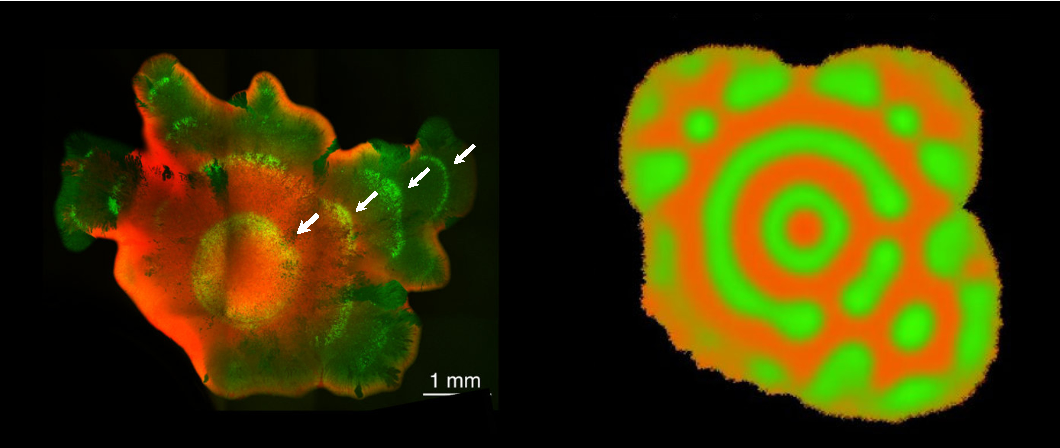
\includegraphics[width=1\textwidth]{chapters/Chapter 3/irregular growth} % The name of your image file; assumes it is in the same directory as your .tex file
    \end{adjustbox}
    \caption{\textbf{Effects of irregular growth in growing colony pattern.} Both in experiment (left) and model (right), more stripes are found in faster-growing fields which form a larger domain}
    \label{fig:irregular growth}
\end{figure}


\subsection{Boundary effects}
The second control involves studying how boundary conditions might affect the resulting pattern.
The boundary conditions at the edge of the colony are always assumed to be absorbing boundary conditions because the diffusors produced in the biofilm get absorbed by the empty agar because of diffusion.
This boundary is indirectly encoded with the masking process (Fig.~\ref{mask}).
However, the boundary at the edge of the simulation square or in other words, where the agar would finish, has to be defined in the ADI numerical solver.
As in Chapter~\ref{Chapter 1}, the absorbing boundaries are introduced by using a Dirichlet boundary condition where the concentration at the boundary is zero $u=0$ as opposed to the previously used Neumann boundaries where the derivative at the boundary is zero.
More details on the encoding of boundaries can be found in Section~\ref{numerical_methods}.
Up to now, all simulations in this Chapter were computed using reflective boundary conditions at the edge of the square.
Here, we introduce absorbing boundary conditions and see that this perturbation leads to fewer rings being produced.
The hypothesis that absorbing boundary conditions make weaker patterns is then tested experimentally.
Absorbing and Reflecting experimental boundaries can be introduced using different sizes of agar plates where the colony grows as seen in Fig.~\ref{fig:boundary_conditions_colony}.
A larger plate will resemble an absorbing boundary condition as we assume diffusors build-up will be less prominent and there will always be a diffusor flux towards the edges of the plate.
On the other hand, a small plate will lead to the quick accumulation of diffusors and therefore these will quickly be reflected as they reach the boundary.
Experimental colonies behave according to model predictions, displaying fewer rings when grown on bigger plates.


\begin{figure}[H] % h! is a placement specifier; it tries to place the image here.
    \centering
    \begin{adjustbox}{center}
        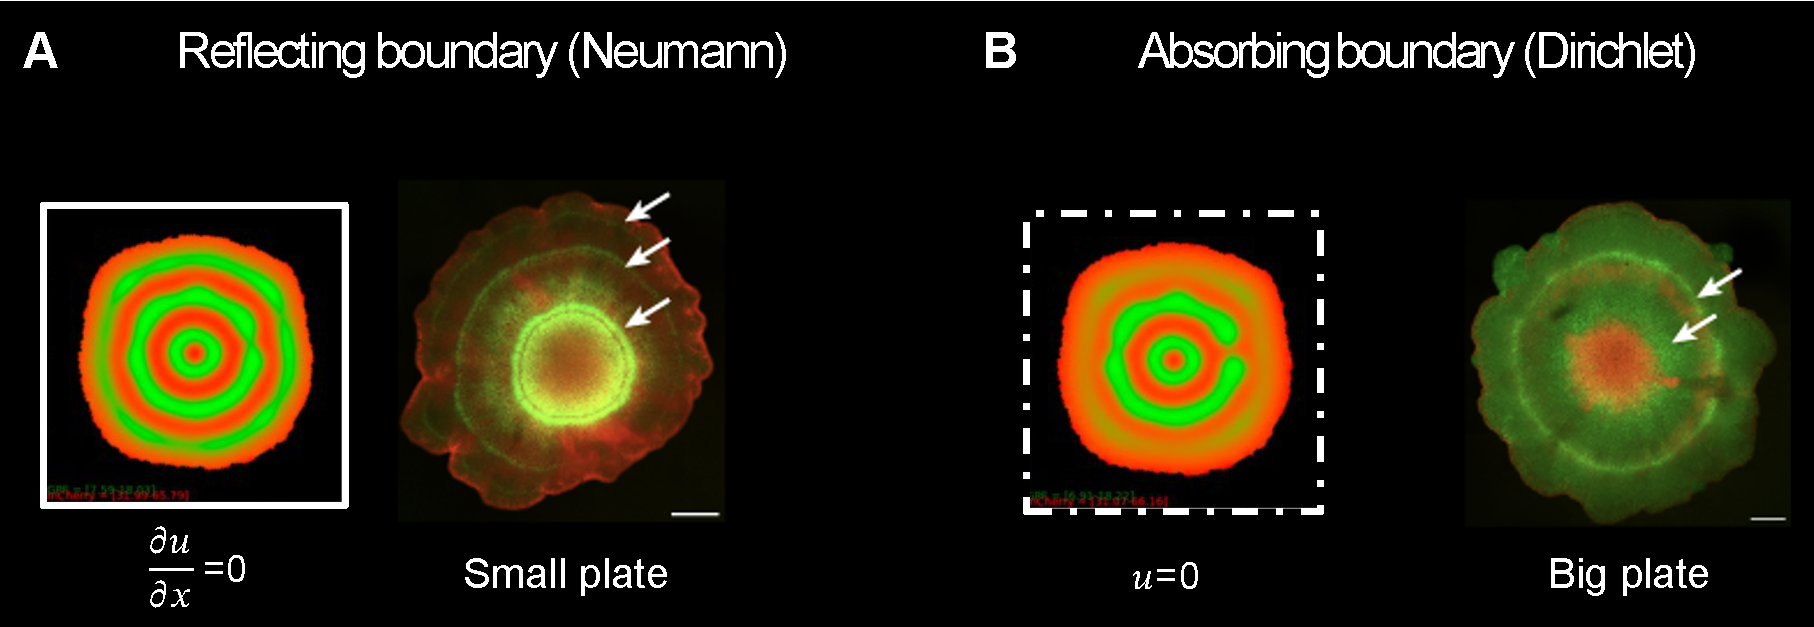
\includegraphics[width=1\textwidth]{chapters/Chapter 3/boundary_conditions_colony} % The name of your image file; assumes it is in the same directory as your .tex file
    \end{adjustbox}
    \caption{\textbf{Effects of boundaries on pattern formation.} The boundary condition affects the patterns. \textbf{(A)} Multiple rings form when cells are grown in smaller wells. Smaller wells are simulated using a reflecting boundary introduced with Neumann boundary conditions. \textbf{(B)} Fewer rings form when grown in larger dishes. Smaller wells are simulated using an absorbing boundary introduced with Dirichlet boundary conditions.}
    \label{fig:boundary_conditions_colony}
\end{figure}

\subsection{Node deletions}
Another important perturbation is deleting nodes of the circuit to study how patterning is affected.
Deletions of each node described in Fig.~\ref{fig:deletion_circuits} were studied using analytical and numerical methods, by re-sampling the parameter space with the literature-based distribution.
The models were defined by taking the original six equation model and removing the following species: RpaI and TetR for Node A deletion, cinI for Node B deletion and cI* for Node C deletion (see Fig.~\ref{fig:deletion_circuits}).

\begin{figure}[H] % h! is a placement specifier; it tries to place the image here.
    \centering
    \begin{adjustbox}{center}
        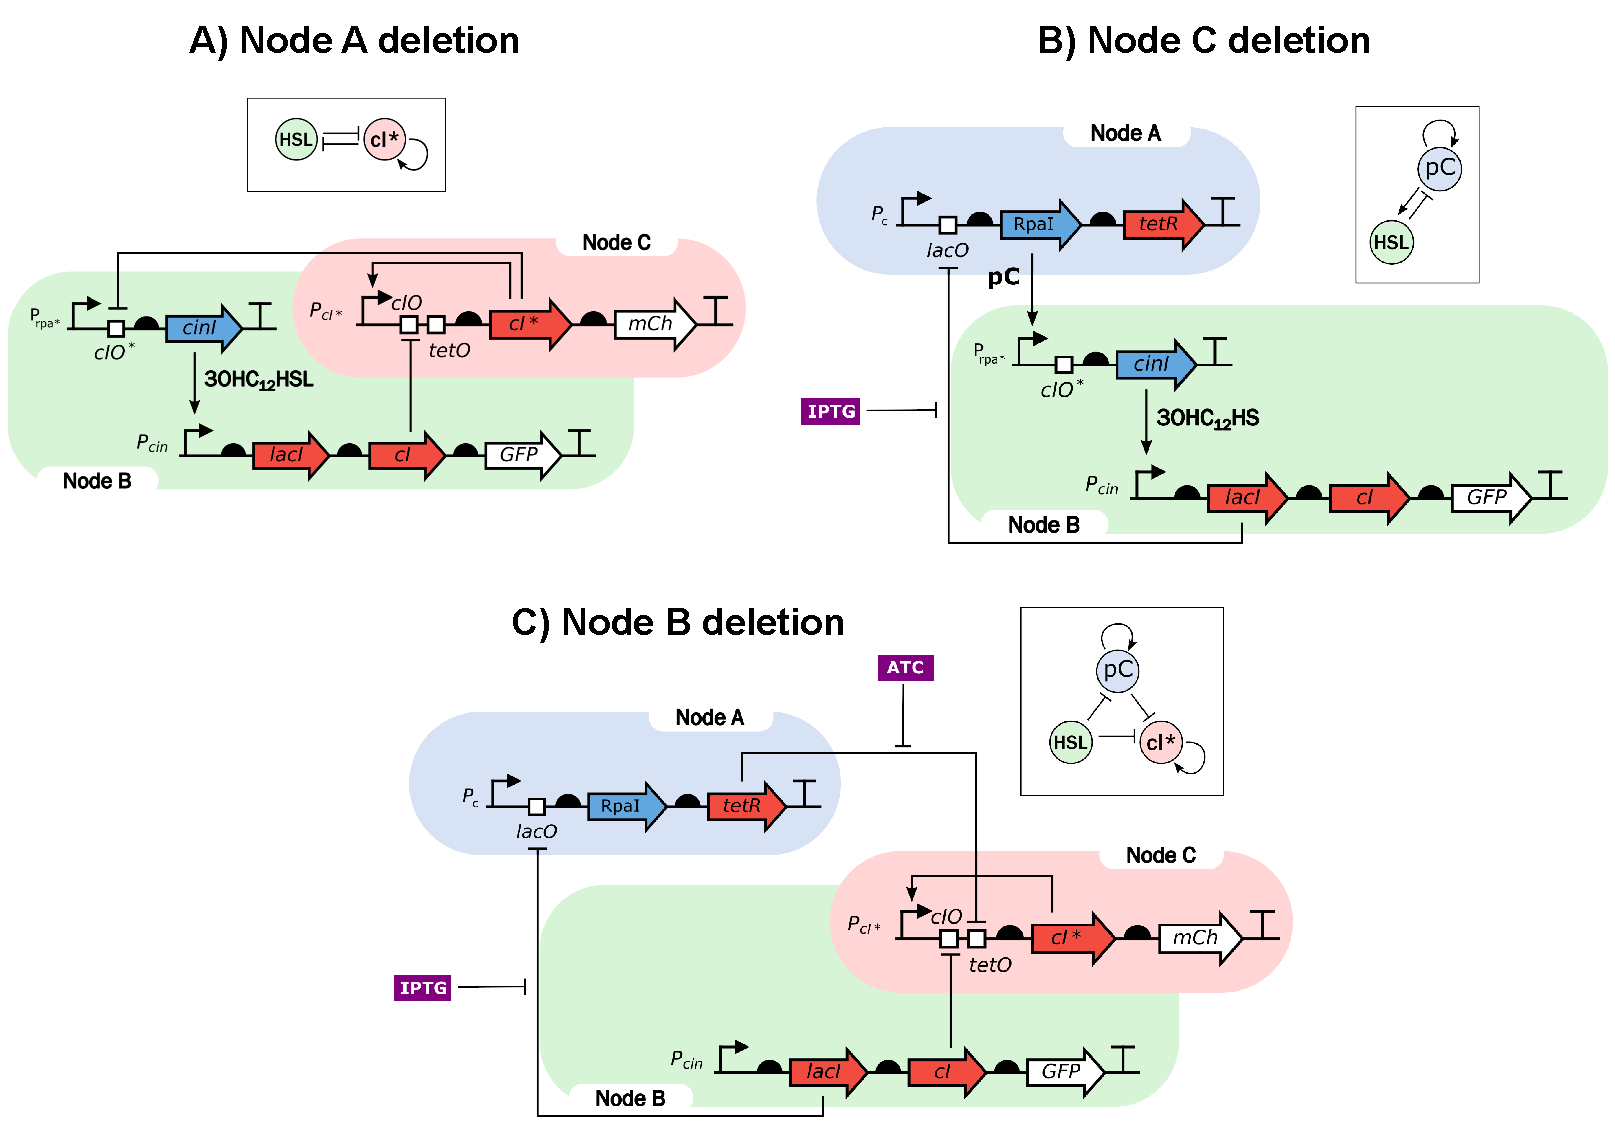
\includegraphics[width=1.1\textwidth]{chapters/Chapter 3/deletion_circuits} % The name of your image file; assumes it is in the same directory as your .tex file
    \end{adjustbox}
    \caption{\textbf{Diagrams of circuit deletions.} \textbf{(A)} Node A deletion involves getting rid of RpaI and tetR genes. This results in a 2 node circuit with a single diffusor. \textbf{(B)} Node B deletion involves removing the cinI gene as well as the inhibition from node C to cinI. This leaves a 3-node circuit with no diffusors regulating gene expression. \textbf{(C)} Node C deletion involves removing cI* and GFP genes, which leads to a 2-node circuit with two diffusors with the original Turing topology.}
    \label{fig:deletion_circuits}
\end{figure}

No Turing I or Turing I Hopf instabilities were found when sampling these three circuits using linear stability analysis.
Some samples were simulated using numerical methods and no periodic patterns were observed either.
Therefore, the model predicts no patterns should arise from the node deletion variants shown in Fig.~\ref{fig:deletion_circuits}.

These variants were then built experimentally and tested by the
Isalan group.
Deletions for node A and node B involve removing the plasmid encoding for that node as in the model.
Deletion for node B involved deleting cinI which is the enzyme producing $OC_{14}$, therefore disconnecting node B from the circuit (Fig.~\ref{fig:deletion_circuits}).
In this variant, node C is deleted too as its only feedback on the circuit is on cinI.
Thin green stripes in the GFP channel, similar to those of the full circuit in Fig.~\ref{fig:outer_ring_addition_modelvsexperiment}, were observed with the three controls after imaging the circuit daily, which produces periodic cold shocks (see Fig.~\ref{fig:experimental_node_dele}).


\begin{figure}[H] % h! is a placement specifier; it tries to place the image here.
    \centering
    \begin{adjustbox}{center}
        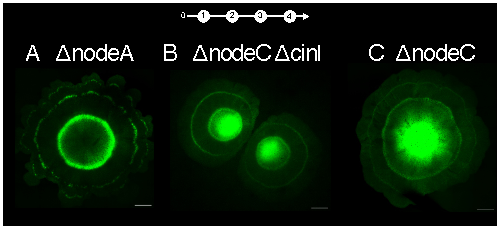
\includegraphics[width=1\textwidth]{chapters/Chapter 3/experimental_node_dele} % The name of your image file; assumes it is in the same directory as your .tex file
    \end{adjustbox}
    \caption{Control experiments testing circuit deletions. All images are taken 4 days after plating, and only the GFP channel is shown. The schematic on top shows on which days a cold-shock has been applied by imaging (white circles). Controls are \textbf{(A)} node A deletion, \textbf{(B)} node B deletion and \textbf{(C)} node C deletion. Images taken by Dr.~Jure Tica}
    \label{fig:experimental_node_dele}
\end{figure}

In this control, the model and experiments disagree as the model does not predict the ring patterns appearing experimentally.
Therefore, these specific rings in the controls cannot be explained with the Turing mechanism and other mechanisms need to be explored.
This suggested that stripe formation was induced by the imaging procedure, possibly because of the drop in temperature during the imaging.
\subsection{Temperature variations}
A potential explanation for the rings is that stripe formation was induced by the imaging procedure, possibly because of the drop in temperature during the imaging.
This hypothesis was not tested with the model because of lack of time.
However, it was explored experimentally by Dr.~Jure Tica and Dr.~Dario Bazzoli and will be shown here for story completeness.

Instead of imaging periodically, the colonies with the full circuit were subjected to cold shocks by putting the plate at room temperature for an hour from the $37^{\circ}$ degree incubator.
First, they cold-shocked the colony every day for four days and four rings were observed on the 5th (see Fig.~\ref{fig:cold_shock_experiments}A).
Then, they only cold-shocked on day one and imaged on day four after plating and this showed three rings (see Fig.~\ref{fig:cold_shock_experiments}B).
Finally, no cold shocks were applied until imaging on day four and no rings appeared as seen in Fig.~\ref{fig:cold_shock_experiments}C.
This proved that periodic cold shocking is not required for periodic patterning, however, a first cold shock on day one is required to get periodic stripes.



\begin{figure}[H] % h! is a placement specifier; it tries to place the image here.
    \centering
    \begin{adjustbox}{center}
        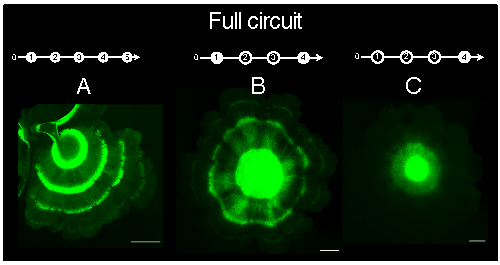
\includegraphics[width=1\textwidth]{chapters/Chapter 3/cold_shock_experiments} % The name of your image file; assumes it is in the same directory as your .tex file
    \end{adjustbox}
    \caption{\textbf{Full circuit experiments under variation of cold shocks.} Green channel of circuit \#1754 exposed to different cold shocks. Cold shocks involve taking the plate out of the incubator for 1h at room temperature. This simulates the cold shock applied to the colony when imaging it in the confocal microscope. Top diagrams show when the cold shocks were applied (white circles), and when they were not (black circles) \textbf{(A)} A cold shock is applied every day for four days, and the image is taken on the 5th day, showing four rings \textbf{(B)} A cold shock is applied only on day one and the image is taken in day four, showing three stripes.  \textbf{(B)} Cold shock is applied only on the 4th day when it is imaged: no rings appear. Images taken by Dr.~Jure Tica}
    \label{fig:cold_shock_experiments}
\end{figure}

To further prove that no periodic cold shocks were needed for periodic patterning, we sought to obtain a time series of the colony while keeping the cells at a constant temperature.
Colonies were grown for a day and then transferred to the microscope, where the first and only cold shock occurred.
The cells were kept at 37°C with a stage-top incubator, and images were taken every hour.
Consistent with the cold shock hypothesis, the first stripe formed soon after the start of the imaging.
Surprisingly, additional stripes formed on the edge of the colony, in parts of the colony with the most prominent outgrowth (Fig.~\ref{fig:microscopy_timeseries}).
Both the timelapse (Fig.~\ref{fig:microscopy_timeseries}) and day1-day4 imaging (Fig.~\ref{fig:cold_shock_experiments}B) show stripes without everyday imaging.
This suggests that after the first stripe is seeded additional stripes can form in a circuit-dependent, reaction-diffusion process.


\begin{figure}[H] % h! is a placement specifier; it tries to place the image here.
    \centering
    \begin{adjustbox}{center}
        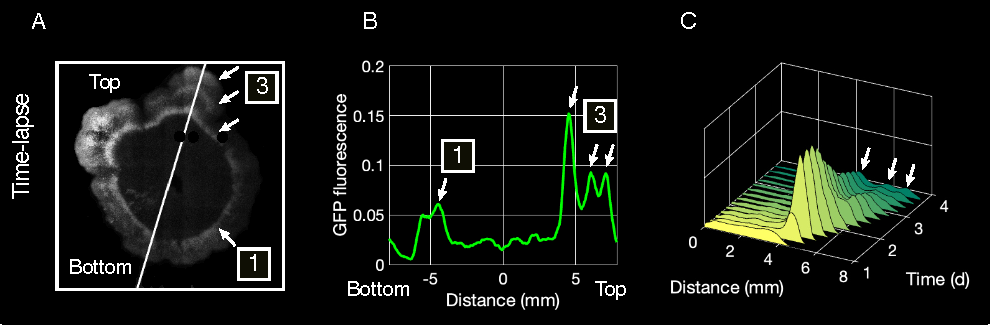
\includegraphics[width=1\textwidth]{chapters/Chapter 3/microscopy_timeseries} % The name of your image file; assumes it is in the same directory as your .tex file
    \end{adjustbox}
    \caption{GFP fluorescence was imaged over 60 hours at a constant temperature of 37 °C. Imaging began after the colony had grown for 24 hours, meaning a single cold shock was applied at 24 hours. \textbf{(A)} The image of the final timepoint shows three stripes in the top right corner of the colony where growth is most prominent (3), and only a single stripe forms at the bottom where there is less growth (1). \textbf{(B)} Plot of the fluorescence along the white slanted line in the micrograph with moving average smoothing. \textbf{(C)} The spatiotemporal profile of GFP evolution shows that the stripes form at the edge of the colony. After an initial burst of fluorescence, the signal decreases over time. Images taken by Dr.~Jure Tica}
    \label{fig:microscopy_timeseries}
\end{figure}



\section{Discussion}

The focus of this chapter was the engineering of patterns in biofilms using the \#1754 topology.
Both experiments and models of synthetic biofilms with spatial patterning were presented.
The overall aim of this chapter was to engineer spatial heterogeneities in biofilms and have a descriptive model to get insights into the patterning mechanisms present.

\subsection{\textit{In-vitro E.~coli} colonies with periodic patterns}
Even though this thesis focused mainly on modelling work, some experimental work was produced to get familiarised with the genetic circuits and the microscopy techniques.
The insights obtained during this work were key to building useful models with accurate assumptions.

During these experiments, the first periodic rings obtained with the \#1754 synthetic circuit were obtained.
These were produced in small colonies with high aTc conditions.
In Chapter~\ref{chapter2}, the model predicted the likelihood of Turing instabilities was higher with high aTc concentrations.
Although it is unclear if the colonies obtained display Turing patterns, aTc did indeed lead to spatial heterogeneities, therefore making the model's predictions useful in guiding the experimental fine-tuning.

The spatial heterogeneities displayed interior ring growth dynamics, where rings were deposited from the inside of the colony and then stretched out (see Fig.~\ref{atcwalk_timeseries_confocal} B).
This behaviour looked similar to the interior ring growth obtained in Hopf instabilities in Fig.~\ref{system_class_simulations} Hopf, top row.
Unlike Turing solutions (Turing I-Hopf and Turing I) where stationary rings were added to the outside, Hopf solutions showed oscillating centres that form into rings in the next step, as in the colonies obtained.
The most likely mechanism behind these specific colonies is therefore probably a Hopf oscillator in a growing colony.
This is also supported by the high probability (4\%) for Hopf solutions in the fine-tuned parameter space (see Fig.~\ref{system_class_frequencies}).

\subsection{Solving PDEs in shaped biofilms}
Following the experimental work produced in this thesis, experimental collaborators explored the system further using larger colonies or biofilms with particular shapes.
A PDE-masking algorithm was built to understand the patterning dynamics of the reaction-diffusion systems in these different biofilm shapes as well as growing domains.
This algorithm is flexible enough that the PDE system can be solved in any mask provided.
Additionally, for complex shapes, image recognition was used to produce this mask as seen in Fig.~\ref{shmoo}.
However, static domains are not the best assumption for growing colonies, as growth may play an important part in tissue dynamics as seen in Chapter~\ref{Chapter 1}.
To encode domain growth into the algorithm, a stochastic cellular automaton was used to produce a growing mask which replicates bacterial colony growth.

One of the caveats of this algorithm is that growth only occurs in the edges and there is no cell death.
In bacterial colonies, although growth is more prominent in the edge, some growth and death also occur in the centre.
Dilution effects were also not taken into account in this algorithm, however, they can be accounted for in the linear degradation terms of the PDE model.
Another issue with the model is that a 2D space was assumed.
Although confocal microscopy only shows a 2D space domain, \textit{E.~coli} colonies have a 3D dome shape~\parencite{wimpenny1979growth}.
Therefore, a 2D snapshot of a 3D model would be more accurate to capture the RD dynamics of the gene circuit.
However, a 2D PDE model was used as it was less computationally expensive.

The PDE model used for these simulations was the six-equation non-dimensional model.
This non-dimensional form of the model makes time and space less intuitive, as these variables have been transformed into non-dimensional.
However, by understanding the parameters of our system we can retransform space and time to their original units: hour and mm.
This transformation is more complicated for space as it is dependent on $D_{U}$, which is sampled from a range.

In terms of spatial resolution, the system was pushed to the smallest $dx$ possible in terms of computational resources.
A pixel of the simulation grid contains around 52-5200~\textit{E.~coli} cells, meaning the system is not discrete at the cell level.
However, we assumed that neighbouring cells have similar dynamics, especially for Turing patterns with larger wavelengths.
Although it is unusual to have a spatial resolution which varies with diffusion rates, the pattern resolution is scaled in the same manner.
A low spatial resolution (e.i. 5200~\textit{E.~coli} per pixel) occurs for large diffusion constants, as well as the pattern wavelength which will be larger with higher diffusion constants.

Overall, this masking method enabled the investigation of Turing patterns in shaped domains.
It was observed that the shape highly affects the resulting Turing patterns obtained when masking the PDE solver with a specific shape.
Throughout this exploration, we saw that Turing patterns tend to form concentric lines following the shape of the biofilm.
This can be an example of how shape conveys morphological robustness to patterning in biology.


\subsection{Replicating bacterial colony patterns}
Using the PDE algorithm masked with the cellular automaton, all patterns obtained experimentally were replicated with the model.
Having documented which types of dispersion relation led to which types of patterns in growing colonies (see Fig.~\ref{system_class_simulations}), we used linear stability analysis to understand the potential mechanisms behind each pattern obtained.
The common red-edge and green-centre pattern (Fig.~\ref{small colony experiment vs model}) could result from any type of dispersion relation, meaning this was a simple boundary effect.
This pattern occurs when diffusers at the edge of the colony get depleted as they leak out onto the agar.
By looking at the circuit (Fig.~\ref{fig:synthetic circuit_chapter2}), we can observe that diffusors are direct GFP activators and mCherry inhibitors.
Therefore, as they get depleted, red is produced and green decays.

Other more complex patterns such as the rings and spots, only appeared in Turing I, Turing I-Hopf and Hopf instabilities (see Fig.~\ref{system_class_simulations}).
More specifically, interior ring growth could be explained with Hopf instabilities while outer ring addition could be explained with Turing I and Turing I-Hopf instabilities.
This coincides with experimental work on Turing patterns in radially growing domains~\parencite{Konow2019}.
In this study, they observed that outer ring addition is the most common Turing pattern growth mode, while interior ring growth in Turing patterns only occurs for extremely slow growth rates.
Labyrinths, which were found in numerical solutions, were not found experimentally.
It is interesting to note that periodic patterns in Turing I-Hopf instabilities occurred more commonly in this model than in Chapter~\ref{Chapter 1}.
This shows how Turing I-Hopf instabilities generate patterns more robustly in certain models or parameter regions.

Another feature of the system which was replicated by the model was the pattern variability or lack of reproducibility.
By searching around the vicinity of a parameter set, many Turing patterns with different shapes could be found.
This could explain why in \textit{in-vitro}, the same experimental conditions led to different pattern outcomes.

Although the outer ring addition and spots obtained can be explained with a Turing mechanism, the robustness of such is extremely low.
Other effects could be increasing the Turing robustness, making this outcome more likely.
For example, colony-induced patterns were observed (see Fig.~\ref{fig:colony_induced_turing}), where the dispersion relation showed no instability but the numerical solution showed periodic spots.
This could be due to the effects of growth, the absorbing boundary conditions or the stochasticity in cell division.
Additionally, it was found that the robustness around a Turing parameter set was extremely high (33.5\% with 1\% uncertainty) compared to the general robustness (0.0025\%) as seen in Fig.~\ref{fig:turing_fit_noise_robustness}A.
Therefore, if by chance the system is explored in experimental conditions that lead to observing a Turing pattern, it is likely to observe another Turing pattern when repeating the experiment under the same conditions.

\subsection{Elucidating mechanisms by modelling experimental controls}
Looking at how different aspects of the pattern compare in the model and in the experiment, can help us elucidate the mechanisms of patterning.
In particular, we aimed to elucidate the mechanism behind the outer ring addition patterns observed in the time-series of Fig.~\ref{fig:outer_ring_addition_modelvsexperiment} top.
The first mechanism that comes to mind is a Turing mechanism, as this produces outer ring addition in our model.
More specifically, a Turing parameter set obtained from the fitted distributions closely replicates the time-series data of the outer ring addition patterns (See Fig.~\ref{fig:outer_ring_addition_modelvsexperiment} bottom).
This means that parameters which are obtained from fitting to liquid-culture experimental data can produce a Turing pattern which resembles our periodic ring patterns.
It is key to mention that the diffusion ratio of this parameter set was the same as the measured diffusion constants in~\cite{tica_diffusers}.
The Turing hypothesis is further strengthened if a Turing parameter set with an experimental diffusion ratio can produce the same experimental rings.

Additionally, several model perturbations applied to this Turing parameter set coincided with the experimental perturbations.
In experiments, faster-growing regions of the colony produced more rings, which was replicated with the irregular growth in the cellular automata algorithm.
Furthermore, more rings were produced in small plates which was replicated by the model using reflecting boundaries as opposed to absorbing boundaries.
This result is reminiscent of~\cite{Krause2020}, where a thick agar layer that absorbed diffusors disrupted Turing patterning.
If perturbations to a Turing model generate the same behaviour in the model as in the experiment, a Turing mechanism is likely behind such a system.

Another perturbation produced was the deletion of nodes, which generated similar concentric as seen in Fig.~\ref{fig:experimental_node_dele}.
Linear stability analysis and numerical simulations determined that such circuits could not produce Turing instabilities.
This suggested rings could be produced by another mechanism such as cold shock effects.
The cold shock hypothesis was tested and indeed it was found that by imaging the colony every day, periodic rings could form as a result of the periodic cold shocks.
The cold shock hypothesis was further proved by the fact that the stripes consistently coincided with the outline of the colony at the previous timepoint (Fig.~\ref{fig:outer_ring_addition_modelvsexperiment}).
If the edges of the colony are more transcriptionally active and the node B promoter or degradation machinery is temperature dependent, a cold shock will induce a temporal overexpression of GFP in the edge of the colony.
If the cells are shocked periodically, a periodic pattern will appear independently of the reaction-diffusion system.

However, time-series experiments and cold shocking at different frequencies of the full circuit showed that periodic rings could still appear without periodic shocking.
Preliminary experiments of the same setup with the circuit deletions did not yield any periodic patterns, suggesting a Turing circuit must be present for those periodic patterns to appear independent of periodic cold shocks.
This suggests that the reaction-diffusion architecture of the gene circuit \#1754 is responsible for the periodic patterning.
However, a pre-pattern seeded by the first cold shock is required for the periodic pattern to occur.
Interestingly, this points to a hybrid Turing and Positional Information mechanism where a pre-pattern provides Turing with an increased robustness to produce periodic patterns.
Future directions involve modelling the \#1754 gene circuit with a pre-pattern to understand whether the robustness for periodic pattern formation increases as this positional information is introduced.

Definitive evidence of Turing patterns would be the emergence of non-symmetrical patterns like regular spots or labyrinths.
However, rings are typically the most prevalent Turing pattern in radially growing domains\parencite{Konow2019}.
The spots observed in Fig.~\ref{comparison_colonies_model_vs_experiment} suggest a patterning mechanism beyond cold shocking due to their asymmetry.
While labyrinths would provide further proof, so far, only rings and spots have been observed in the sampled fitted parameter distributions and in the experiments.


